\documentclass{ximera}

\graphicspath{{./}{eulerCharacteristic}}


\title{Euler Characteristic, Part 2}
\author{Bart Snapp \and Brad Findell}
\begin{document}
\begin{abstract}
In this activity we are going to further investigate some fundamental
properties of shapes.
\end{abstract}
\maketitle


%\begin{question}[3in]
%Last time we drew a number of figures, counted their vertices, edges, and faces, and recorded the results in a table.  Give some examples. 
%\begin{freeResponse}
%\end{freeResponse}
%\end{question}
%
%
%\begin{question}[2in]
%What patterns and relationships do you see among the numbers of vertices, edges, and faces?
%\begin{freeResponse}
%\end{freeResponse}
%\end{question}
%
%
%\begin{question}[3in]
%In order to explain the patterns and relationships, we need careful definitions of vertices, faces, and edges.  Write some definitions.  
%\begin{freeResponse}
%\end{freeResponse}
%\end{question}
%
%
%
%\begin{question}
%Provide a summary of what we were able to conclude.
%\begin{freeResponse}
%\end{freeResponse}
%\end{question}
%
\begin{question}
Last time we drew a number of figures, counted their vertices ($V$), edges ($E$), and faces ($F$), and recorded the results.  We noticed that it the equation $V-E+F=1$ was usually true.  It was obviously true for a polygon with $n$ sides: $V=n$, $E=n$, and $F=1$, so $V-E+F=n-n+1=1$.  

But because the equation was sometimes not true, we decided needed better definitions and rules about vertices faces, and edges.  Most of you proposed definitions on Carmen.  Many of them were of the following form: 
\begin{itemize}
\item A vertex is [something about] edges. 
\item An edge is [something about] vertices or faces. 
\item A face is [something about] edges. 
\end{itemize}
\begin{enumerate}
\item Why are such definitions sometimes called ``circular''?  
\item Describe why ``circular'' definitions can be problematic. 
\item Describe a better approach to defining three related terms.  
\end{enumerate}
\begin{freeResponse}
\end{freeResponse}
\vfill
\end{question}
\newpage

\begin{question}
It turns out to be quite useful to \textbf{classify} figures by their value of the expression 
$V-E+F$.  Below each figure, write the expression $V-E+F$ and compute its value.  
\begin{itemize}
\item If there is any ambiguity about where a vertex might be, make an obvious dot.  
\item If a figure seems to be ``against the rules,'' then draw \textbf{additional} vertices, edges, or faces to correct it.  
\end{itemize}
\[
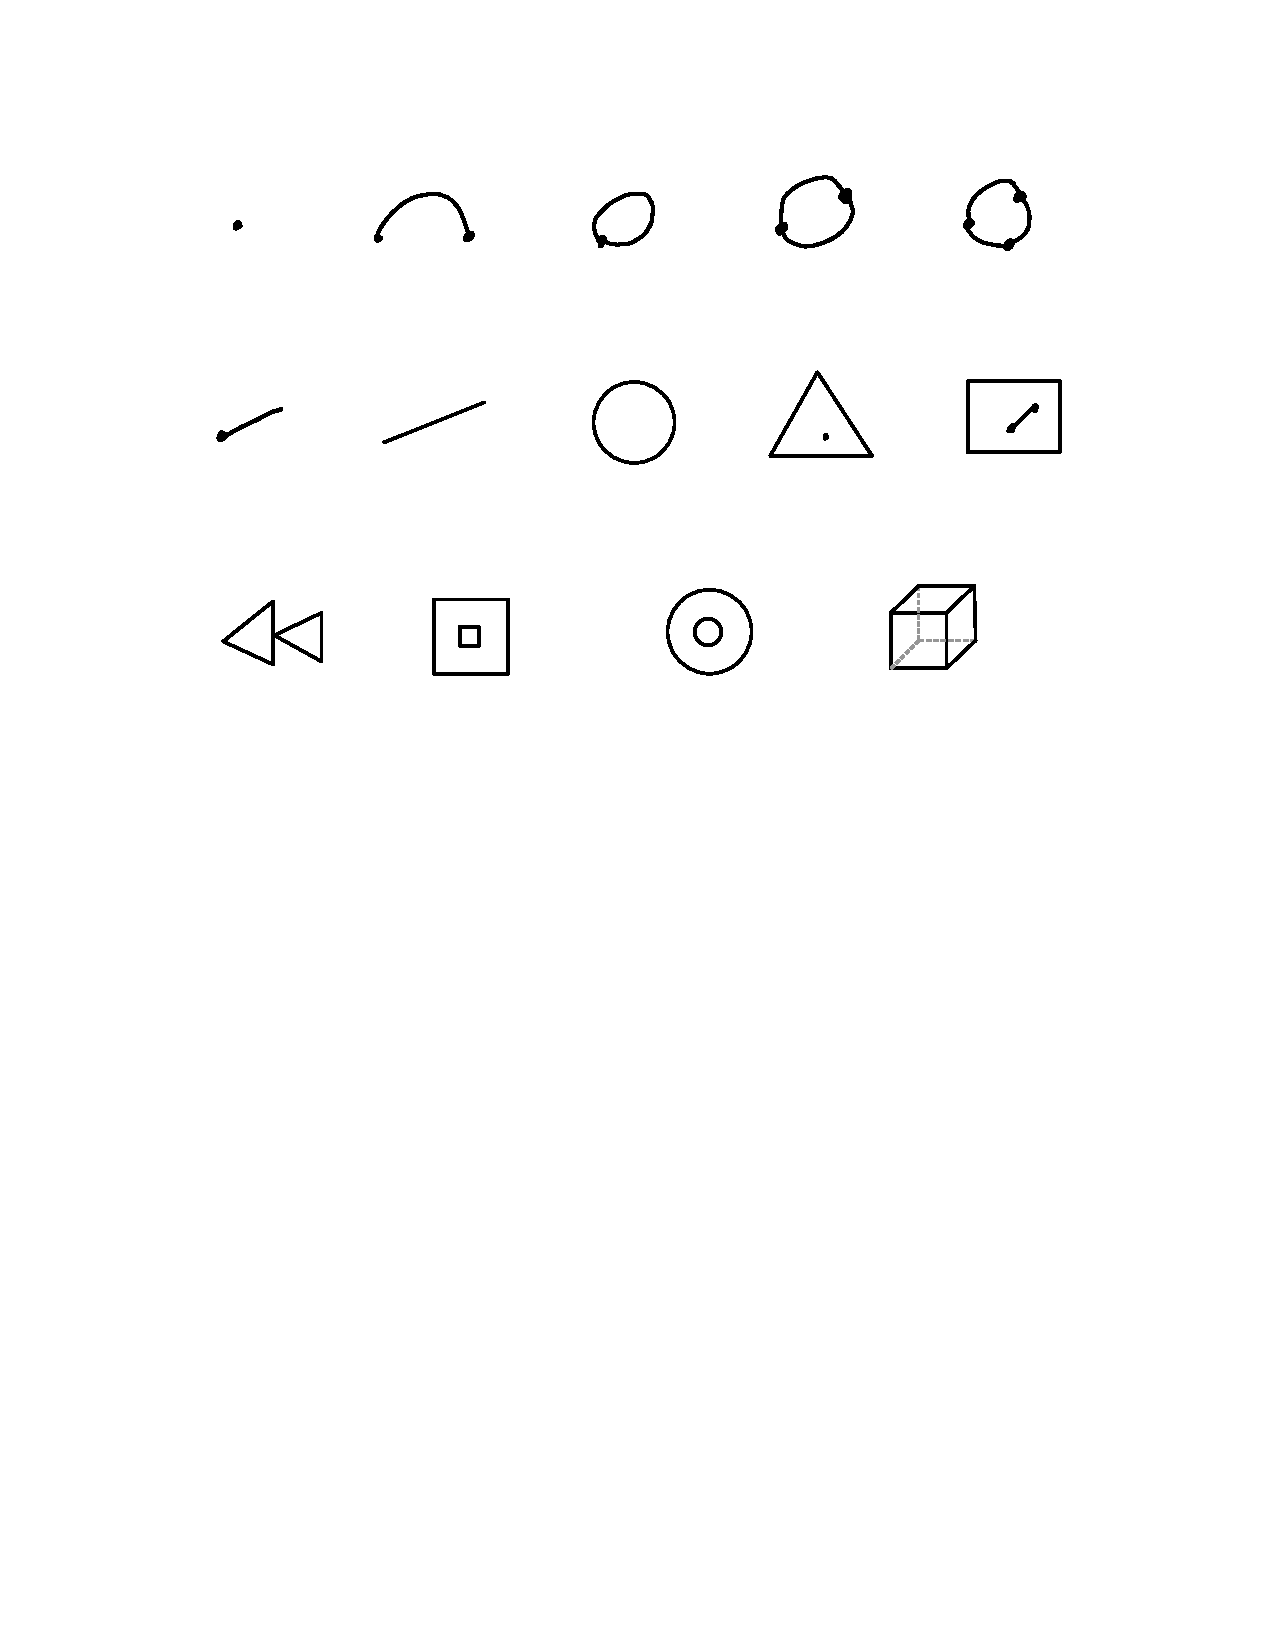
\includegraphics{eulerFigures.pdf}
\]
\vspace{0.5in}

Add some of your own figures.  
\begin{freeResponse}
\end{freeResponse}
\vfill
\end{question}

\newpage

\begin{question}
Now write definitions of vertices, edges, and faces that you think will work for all of your corrected versions of the previous figures.  
\begin{freeResponse}
\end{freeResponse}
\vfill
\end{question}


\end{document}





